\chapter{Scripts and Live Scripts}

So far we've typed all of our programs ``at the prompt.'' If you're only writing a few lines, this isn't so bad. But what if you're writing a hundred? Retyping each line of code every time you want to change or test your program will be time-consuming and tedious. Luckily, you don't have to. In this chapter, we'll look at two ways to run many lines at once: \emph{scripts} and \emph{live scripts}.

\section{Scripts}

A \emph{script} is a file that contains MATLAB code. When you run a script, MATLAB executes the commands in it, one after another, exactly as if you had typed them at the prompt. Scripts are
also sometimes called \emph{M-files} because they use the extension \emph{.m}, short for MATLAB.

\index{script}
\index{M-file}
\index{file extension}

\subsection{Your First Script}

You can create scripts with any text editor or word processor, but the simplest way is to click the \textbf{New->Script} button in the upper-left corner of the MATLAB interface, which opens a text editor designed for MATLAB, simpl;y called the "Editor".

To try it out, create a new script and enter the following code:

\begin{code}
x = 5
\end{code}

Then press the \textbf{Save} button.  A dialog window should appear where you can choose the filename and the folder where your script will go.
Change the name to \emph{myscript.m} and save it into any folder you like.

Now click the green \textbf{Run} button.  You might get a message that says the script is not found in the current folder.
If so, click the button that says Change Folder and it should run.  

A handy way to discover the current folder in which the Command Window is operating is to issue the \lstinline{pwd} command - for 'print working directory'.  You can also issue the \lstinline{ls} command to display a listing of the files and folders in the current working directory, for example
\begin{code}
  >> ls
bike_update.m	     fibonacci1_live.pdf  mylivescript.mlx  myscript.m
fibonacci1_live.mlx  fibonacci1.m	  mylivescript.pdf  swap.m
\end{code}

\index{Command Window}

\textbf{Pro Tip:} You will likely find you run scripts, or portions of a script, frequently while you are developing, testing and debugging.  The keyboard shorcuts can speed up this interation cycle.  To run the entire script the \textbf{F5} key is equivalent to clicking the Run button and to typing the name of the script in the Command Window.  To run just a portion of your script, highlight that section and press the \textbf{Ctrl+Enter} keys.

You can also run a script by typing its name in the Command Window and pressing \keycap{enter}. For example, if you enter \lstinline{myscript}, MATLAB should execute your script and display the result:

\begin{code}
>> myscript
x = 5
\end{code}

There are a few things to keep in mind when using scripts. First, you should not include the extension \emph{.m} when you run a script.  If you do, you'll get an error message like this:

\begin{code}
>> myscript.m
Undefined variable "myscript" or class "myscript.m".
\end{code}

Second, when you name a new script, try to choose something meaningful and memorable.
Don't choose a name that's already in use; if you do, you'll replace one of MATLAB's functions with your own (at least temporarily).
You might not notice right away, but you might get some confusing behavior later.

\index{script!filename}

Also, the name of the script cannot contain spaces.  If you create
a file named \emph{my script.m}, MATLAB will complain when you try
to run it:

\begin{code}
>> my script
Undefined function or variable 'my'.
\end{code}

It can be hard to remember which folder a script is in.  To keep things simple,
for now, I suggest putting all of your scripts in one folder.

\subsection{Why Scripts?}

There are a few good reasons to use a script. When you're writing more than a couple of lines of code, it might take a few tries to get everything right.  Putting your code
in a script makes it easier to edit than typing it at the prompt. Likewise, if you're running a script repeatedly, it's much faster to type the name of the script than to retype the code! And you might be able to reuse a script from one project to the next, saving you considerable time across projects.

\index{script!reasons for}


But the great power of scripts comes with great responsibility: you have to make sure that the code you are running is the code you think you are running.
Whenever you start a new script, start with something simple, like \lstinline{x = 5}, that produces a visible effect. Then run your script and confirm that you get what you expect.
When you type the name of a script, MATLAB searches for the script in a \emph{search path}, which is a sequence of folders.  If it doesn't find the script in the first folder, it searches the second, and so on.
If you have scripts with the same name in different folders, you could be looking at one version and running another.

\index{search path}
\index{folder}

\index{debugging!Third Theorem}

If the code you are running is not the code you are looking
at, you'll find debugging a frustrating exercise!  So it's no surprise that this is the Third Theorem of Debugging:

\begin{quote}
Be sure that the code you are running
is the code you think you are running.
\end{quote}

Now that you've seen how to write a script, let's use one to do something a little more complicated.

\subsection{Example: The Fibonacci Sequence}

\index{Fibonacci number}
\index{sequence!Fibonacci}

The \emph{Fibonacci sequence}, denoted $F$, is a sequence of numbers where each number is the sum of the previous two.
It's defined by the equations $F_1 = 1$, $F_2 = 1$, and, for $i > 2$, $F_{i} = F_{i-1} + F_{i-2}$.
The following expression computes the $n$th Fibonacci number:
%
\begin{equation*}
F_n = \frac{1}{\sqrt{5}}
\left[
\left( \frac{1 + \sqrt{5}}{2} \right)^{n} -
\left( \frac{1 - \sqrt{5}}{2} \right)^{n}
\right]
\end{equation*}
%

We can translate this expression into MATLAB, like this:

\begin{code}
s5 = sqrt(5);
t1 = (1 + s5) / 2;
t2 = (1 - s5) / 2;
diff = t1^n - t2^n;
ans = diff / s5
\end{code}

I use temporary variables like \lstinline{t1} and \lstinline{t2} to make the code readable and the order of operations explicit.  The first four lines have a semicolon at the end, so they don't display anything.  The last line assigns the result to \lstinline{ans}.

\index{semicolon}

If we save this script in a file named \emph{fibonacci1.m}, we can run it like this:

\begin{code}
>> n = 10
>> fibonacci1
ans = 55.0000
\end{code}

Before calling this script, you have to assign a value to \lstinline{n}.
If \lstinline{n} is not defined, you get an error:

\begin{code}
>> clear n
>> fibonacci1
Undefined function or variable 'n'.

Error in fibonacci1 (line 9)
diff = t1^n - t2^n;
\end{code}

This script only works if there is a variable named \lstinline{n} in the workspace; otherwise, you should get an error.
MATLAB will tell you what line of the script the error is in and display the line.

\index{workspace}

\index{debugging!Fourth Theorem}

Error messages can be helpful, but beware!
In this example, the message says the error is in \lstinline{fibonacci}, but the actual problem is that we have not assigned a value to \lstinline{n}.
And that brings us to the Fourth Theorem of Debugging:

\begin{quote}
Error messages tell you where the problem was discovered,
not where it was caused.
\end{quote}

Often you have to work backwards to find the line of code (or missing line) that caused the problem.

\subsection{Floating-Point Numbers}

In the previous section, the result we computed was \lstinline{55.0000}.  Since the Fibonacci numbers are integers, you might have been surprised to see the zeros after the decimal point.

They are there because MATLAB performs calculations using floating-point numbers.  With \emph{floating-point numbers}, integers can be represented exactly, but most fractions cannot.

\index{floating-point}
\index{number!floating-point}

For example, if you compute the fraction 2/3, the result is only approximate---the correct answer has an infinite number of 6s:

\begin{code}
>> 2/3
ans = 0.6666
\end{code}



It's not as bad as this example makes it seem: MATLAB uses more digits than it shows by default.
You can use the \lstinline{format} command to change the output format:

\index{format@\lstinline{format}}

\begin{code}
>> format long
>> 2/3
ans = 0.666666666666667
\end{code}

In this example, the first 14 digits are correct; the last one has been rounded off.

\index{scientific notation}
\index{factorial@\lstinline{factorial}}

Large and small numbers are displayed in \emph{scientific notation}.
For example, if we use the built-in function \lstinline{factorial} to compute $100!$, we get the following result:

\begin{code}
>> factorial(100)
ans = 9.332621544394410e+157
\end{code}

The \lstinline{e} in this notation is \emph{not} the transcendental number
known as $e$; it's just an abbreviation for ``exponent.''  So
this means that $100!$ is approximately $9.33 \times 10^{157}$.  The
exact solution is a 158-digit integer, but with double-precision floating-point numbers, we only know the first 16 digits.

\index{transcendental number}
\index{exponent}

You can enter numbers using the same notation.

\begin{code}
>> speed_of_light = 3.0e8
speed_of_light = 300000000
\end{code}

Although the floating-point format can represent very large and small numbers,
there are limits.
The predefined variables \lstinline{realmax} and \lstinline{realmin}
contain the largest and smallest numbers MATLAB
can handle.

\index{realmin@\lstinline{realmin}}
\index{realmax@\lstinline{realmax}}

\begin{code}
>> realmax
ans = 1.797693134862316e+308

>> realmin
ans = 2.225073858507201e-308
\end{code}

If the result of a computation is too big, MATLAB ``rounds up''
to \mbox{infinity}.

\index{Inf@\lstinline{Inf}}

\begin{code}
>> factorial(170)
ans = 7.257415615307994e+306

>> factorial(171)
ans = Inf
\end{code}

Division by zero also returns \lstinline{Inf}.

\begin{code}
>> 1/0
ans = Inf
\end{code}

\index{division!by zero}
\index{zero!division by}

For operations that are undefined, MATLAB returns \lstinline{NaN},
which stands for ``not a number.''

\index{NaN@\lstinline{NaN}}
\index{not a number}
\index{undefined operation}

\begin{code}
>> 0/0
ans = NaN
\end{code}


\subsection{Comments}

Short, simple programs are easy to read, but as they get bigger and more complex, it gets harder to figure out what they do and how.  That's what comments are for.

A \emph{comment} is a line of text added to a program to explain how it works. It has no effect on the execution of the program; it is there for human readers.
Good comments make programs more readable; bad comments are useless at best and misleading at worst.

To write a comment, you use the percent symbol (\%) followed by the text of the comment.

\index{comment}
\index{\%@\lstinline{\%}}
\index{percent sign}

\begin{code}
>> speed_of_light = 3.0e8     % meters per second
speed_of_light = 300000000
\end{code}

The comment runs from the percent symbol to the end of the line.
In this case it specifies the units of the value.  In an ideal world,
MATLAB would keep track of units and propagate them through the
computation, but for now that burden falls on the programmer.

\index{unit}

Avoid comments that are redundant with the code:

\begin{code}
>> x = 5        % assign the value 5 to x
\end{code}

Good comments provide additional information that's not in the
code, like units in the example above, or the meaning of a variable:

\begin{code}
>> p = 0         % position from the origin in meters
>> v = 100       % velocity in meters / second
>> a = -9.8      % acceleration of gravity in meters / second^2
\end{code}

If you use longer variable names, you might not need explanatory
comments, but there's a trade-off: longer variable names are clearer, but longer code can become harder
to read.
Also, if you're translating from math
that uses short variable names, it can be useful to make your
program consistent with your math.

\index{variable name}

\subsection{Documentation}

Every script should provide \emph{documentation}, which is a comment
that explains what the script does and what its requirements are.

For example, I might put something like this at the beginning of \emph{fibonacci1.m}:

\index{documentation!function}
\index{function!documentation}

\begin{code}
% Computes a numerical approximation of the nth Fibonacci number.
% Precondition: you must assign a value to n before running this script.
% Postcondition: the result is stored in ans.
\end{code}

A \emph{precondition} is something that must be true when the script
starts in order for it to work correctly.  A \emph{postcondition}
is something that will be true when the script completes.

\index{precondition}
\index{postcondition}
\index{Fibonacci}

If there is a comment at the beginning of a script, MATLAB assumes
it's the documentation for the script. So if you type \lstinline{help fibonacci1}, you get the contents of the comment (without the percent
signs).

\begin{code}
>> help fibonacci1
  Computes a numerical approximation of the nth Fibonacci number.
  Precondition: you must assign a value to n before running this script.
  Postcondition: the result is stored in ans.
\end{code}

That way, scripts that you write behave just like predefined scripts.
You can even use the \lstinline{doc} command to see your comment in the
Help Window.

\index{Help Window}
\index{doc@\lstinline{doc}}
\index{help@\lstinline{help}}

\subsection{Assignment and Equality}

For beginning programmers, a common source of confusion is assignment and the use of the equals sign.

\index{variable!assignment}
\index{assignment!target}
\index{equality}

In mathematics, the equals sign means that the two sides of the
equation have the same value.
In MATLAB, an assignment statement \emph{looks} like a mathematical equality, but it's not.

One difference is that the sides of an assignment statement are not
interchangeable.  The right side can be any legal expression, but
the left side has to be a variable, which is called the
\emph{target} of the assignment.  So this is legal:

\begin{code}
>> y = 1;
>> x = y + 1
x = 2
\end{code}

But this is not:

\begin{code}
>> y + 1 = x
 y + 1 = x
       |
Error: Incorrect use of '=' operator.
To assign a value to a variable, use '='.
To compare values for equality, use '=='.
\end{code}

In this case the error message is not very helpful.  The problem here is that the expression on the left side is not a valid target for an assignment.

\index{error message}

Another difference between assignment and equality is that a mathematical equality is true (or false) for all eternity;
an assignment statement is temporary.
When you assign \lstinline{x = y + 1}, you get the
\emph{current} value of \lstinline{y}.  If \lstinline{y} changes later, \lstinline{x}
does not get updated.

A third difference is that a mathematical equality is a statement that
may or may not be true.  In mathematics, $y = y+1$ is a statement that
happens to be false for all values of $y$.
In MATLAB, \lstinline{y = y + 1} is a sensible and useful assignment statement.
It reads the current value of \lstinline{y}, adds 1, and replaces the old value with the new value.

\begin{code}
>> y = 1;
>> y = y + 1
y = 2
\end{code}

When you read MATLAB code, you might find it helpful to pronounce
the equals sign as ``gets'' rather than ``equals.''  So \lstinline{x = y + 1}
is pronounced ``\lstinline{x}~gets the value of \lstinline{y} plus one.''

\section{Live Scripts}

A MATLAB \emph{live script} is an interactive document that combines code, formatted text (e.g., equations), images and output in once place.  In one sense it merges the code from a script with the execution of the command window.  A live script allows you to run sections of your program independently, debugging as you go, while embedding the computation in a portable document that you can export and share.

\subsection{Your First Live Script}

While regular (non-live) scripts are stored as a text file with the \emph{.m} extension, live scripts are stored as package of code, rich text and images.   Luckily, MATLAB hides all this complexity from the user and what you see is a single document, stored as a \emph{.mlx} file.

You can create a live script by clicking the \textbf{New->Live Script} button in the upper-left corner of the MATLAB interface.  This opens the MATLAB "Live Editor".  Create a new live script and add the following:

\begin{enumerate}
\item Add a text block.  This is rich text that can be formatted using the buttons on the top of the Live Editor or using \href{https://www.mathworks.com/help/matlab/matlab_prog/format-live-scripts.html}{markdown}.
\item Add a code block with the line \lstinline{x = 5}.
\end{enumerate}

Then press the \textbf{Save} button to save the file as \emph{mylivescript.mlx}.

Now click the same green \textbf{Run} button (or hit F5) to run the scipt and see the result in the same document.  You can still call the live script from the Command Window:
\begin{code}
  >> mylivescript
  x =
       5
\end{code}
But that is probably a rare use-case.

In addition to saving the live script as an \emph{.mlx} file, you can also export the document in a variety of formats.  Here is what the a PDF export might look like:


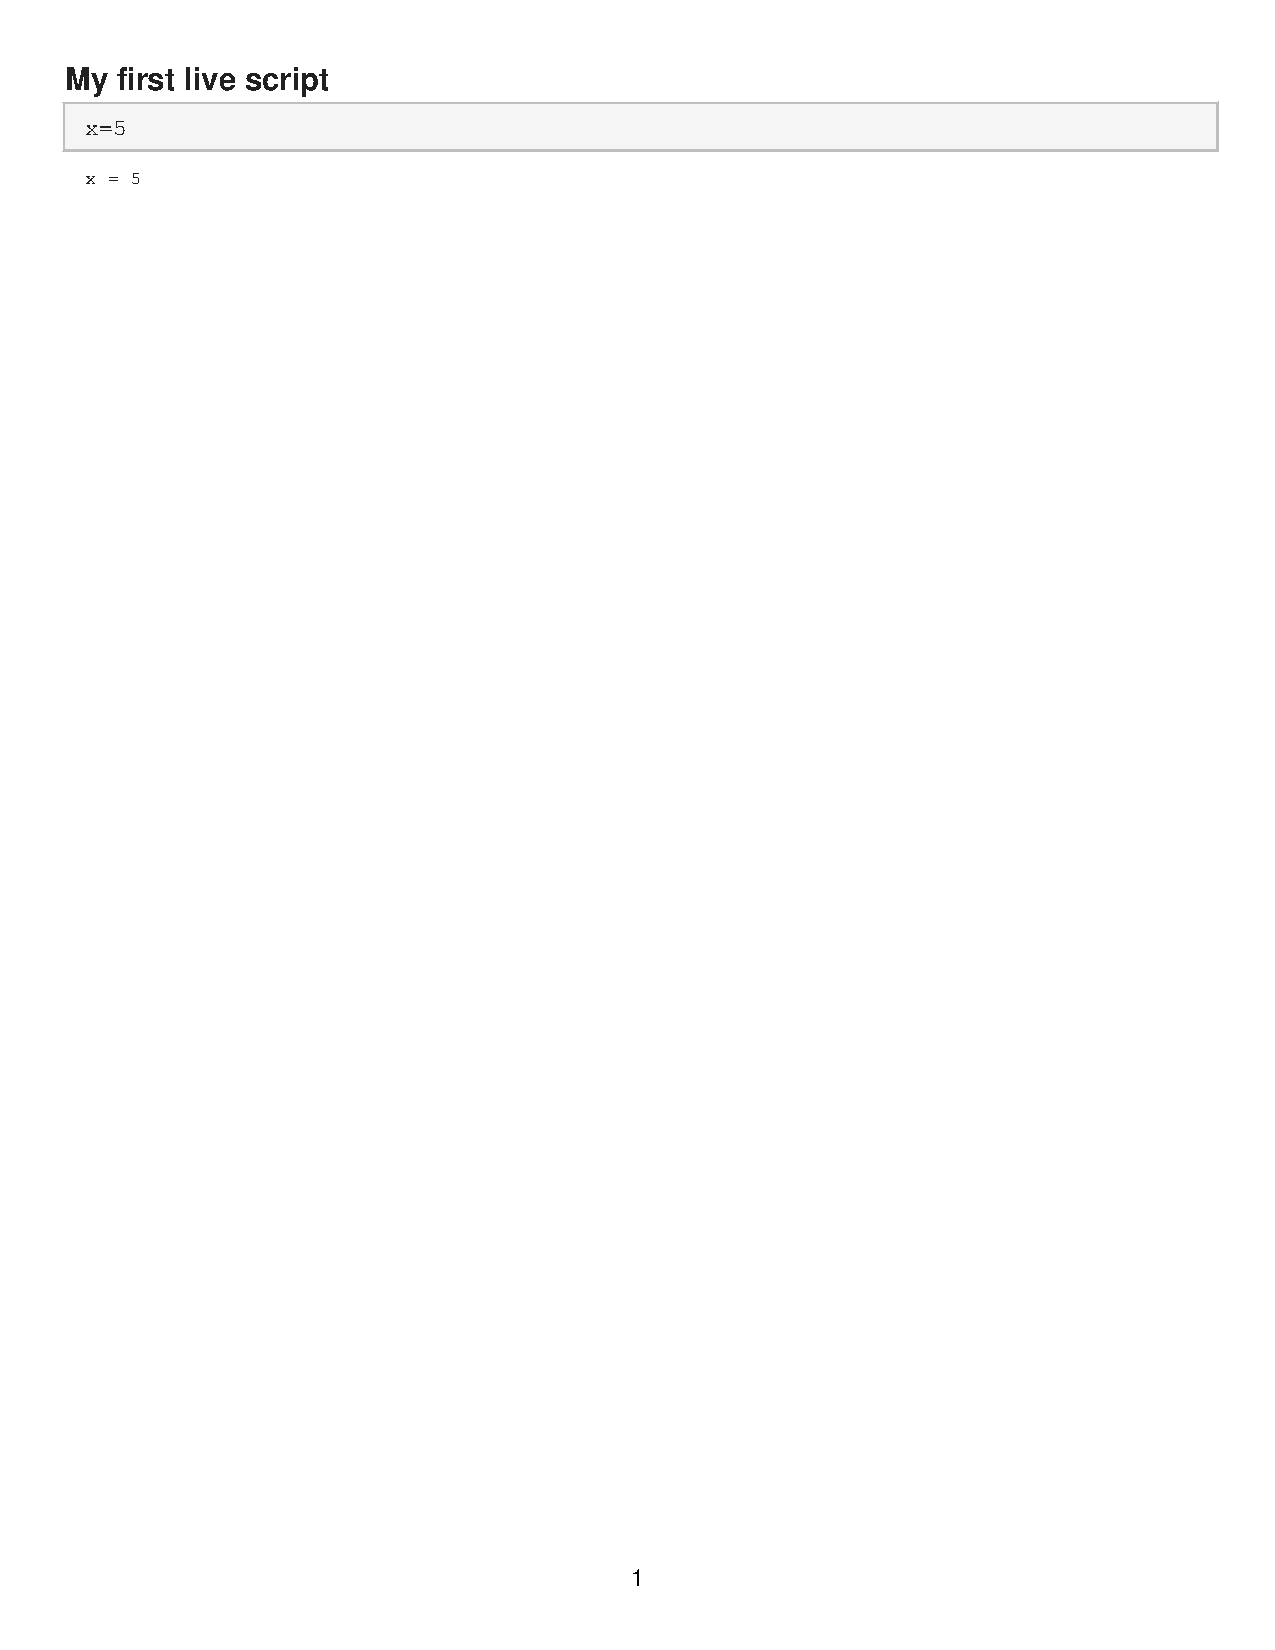
\includepdf[pages=-,frame,pagecommand={},width=0.9\textwidth]{../code/chap_scripts/mylivescript.pdf}

\subsection{Example: The Fibonacci Sequence}

Returning to our earlier example of a plain script, we can now combine the rich text of the description, inlcuding the expression for the Fibonacci number, into a live script with alternating text and code blocks.  The resulting PDF would look something like this: 

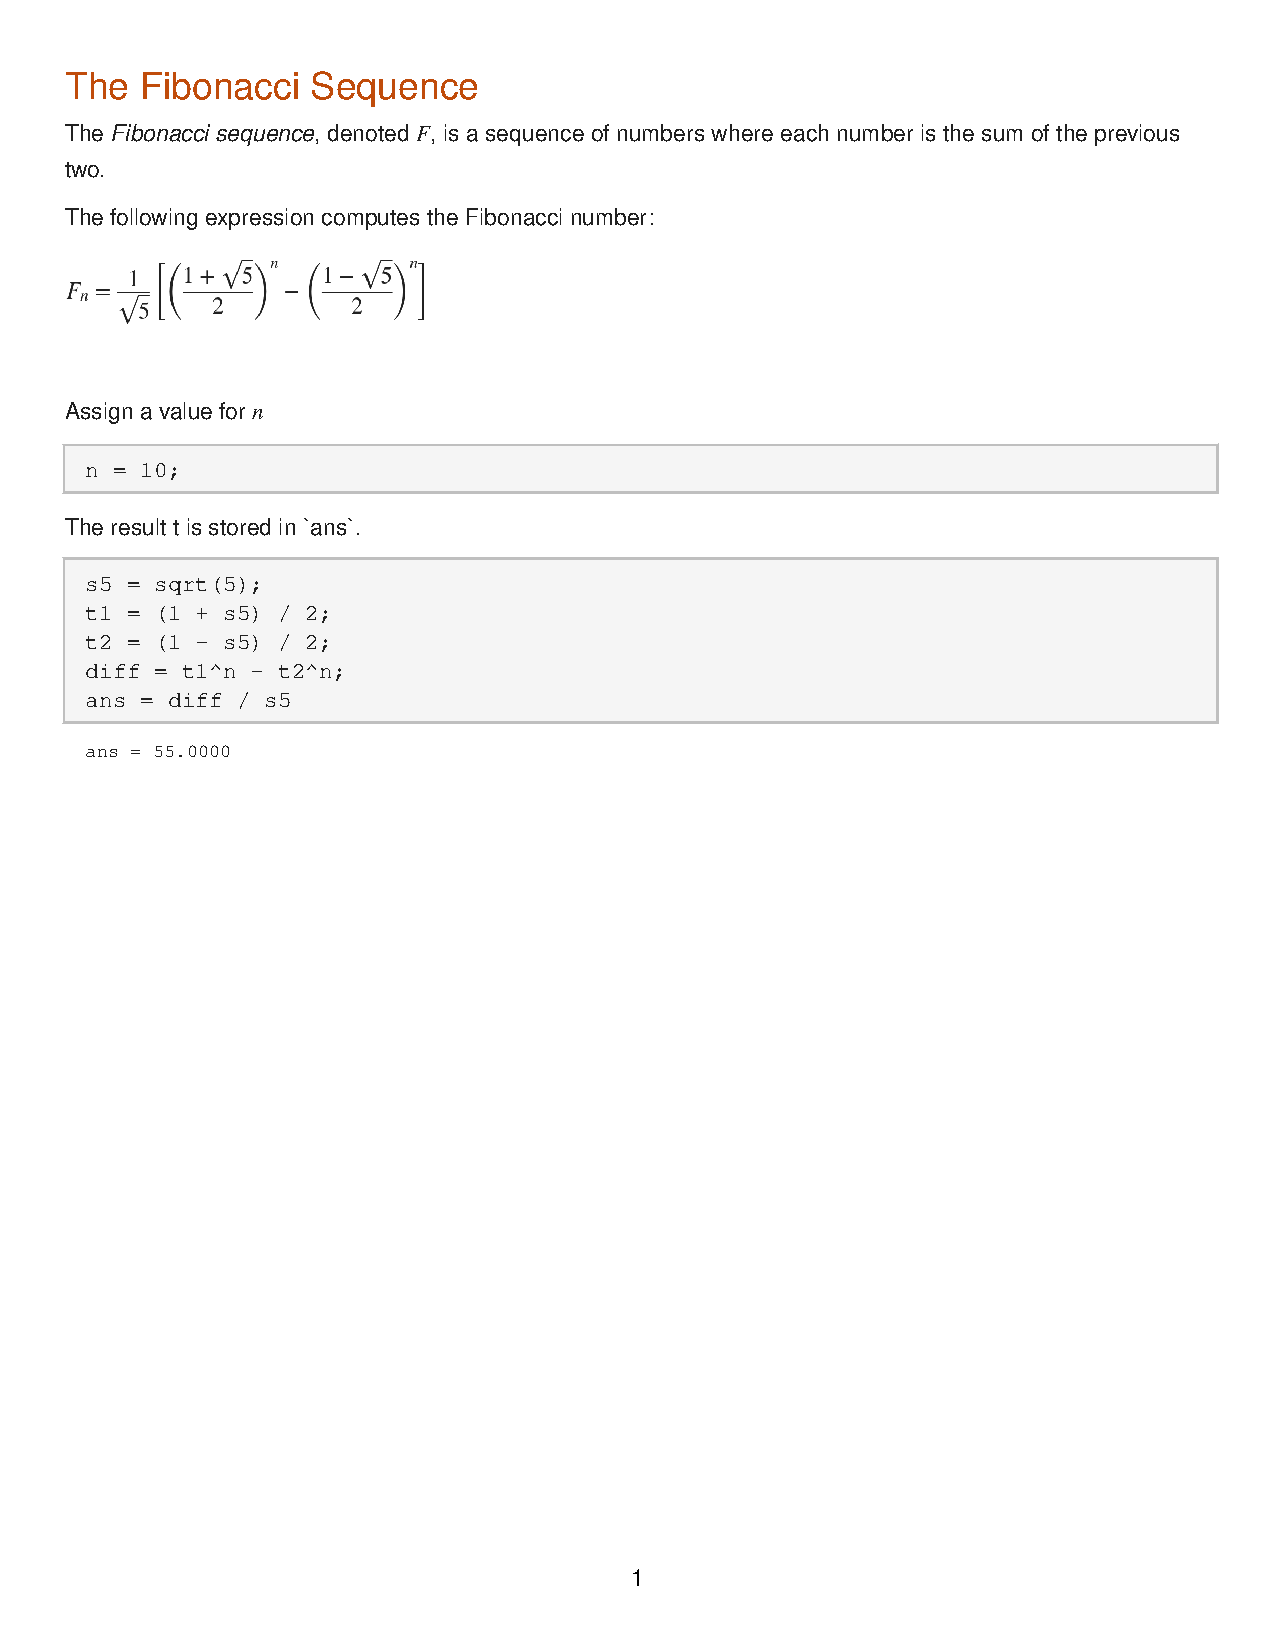
\includepdf[pages=-,frame,pagecommand={},width=0.9\textwidth]{../code/chap_scripts/fibonacci1_live.pdf}
%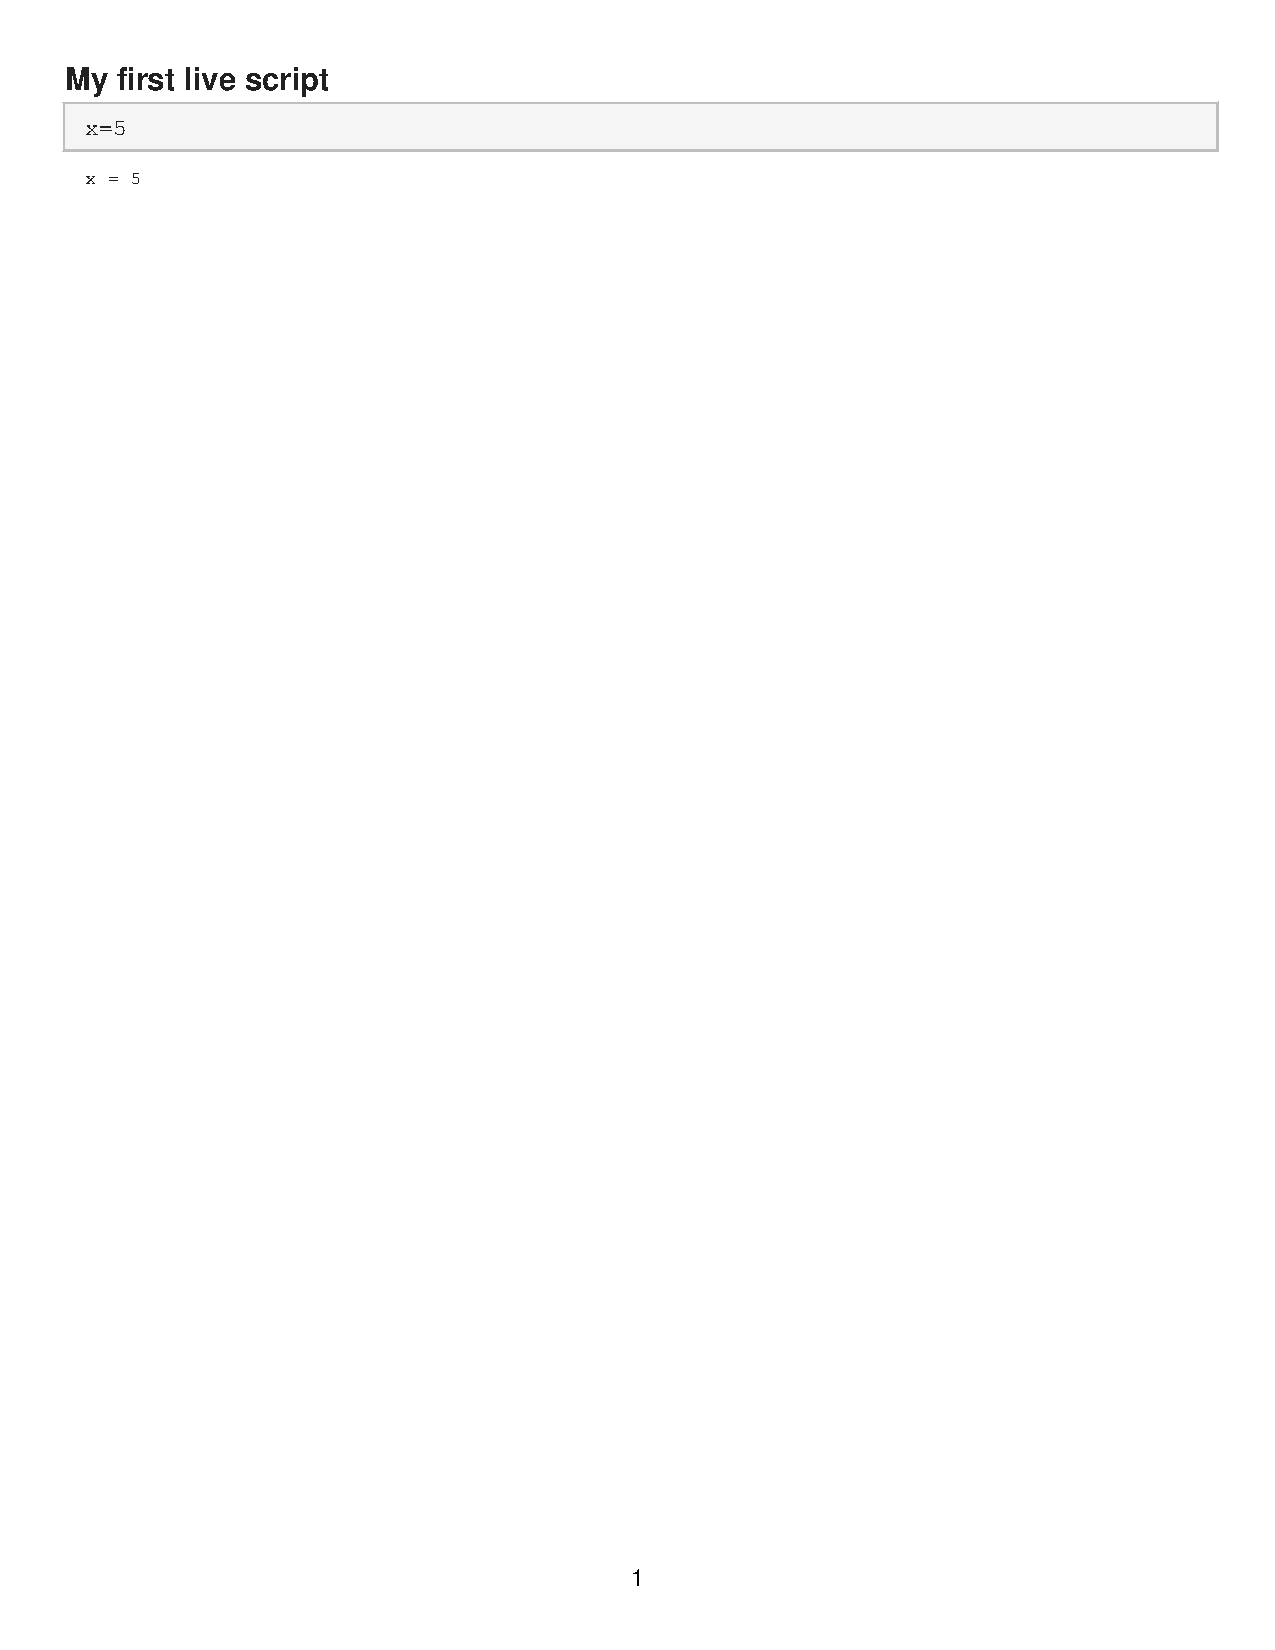
\includepdf[pages=-,frame,pagecommand={},width=0.9\textwidth]{../code/chap_scripts/mylivescript.pdf}

\section{Chapter Review}

This chapter presented scripts and live scirpts, suggesting reasons to use them.  We computed elements of a Fibonacci sequence, but because we used floating-point numbers, the results were sometimes only approximate.
And we saw how to add comments to a program to document what it does and explain how it works.

Here are some terms from this chapter you might want to remember.

An \emph{M-file} is a file that contains a \emph{script}, which is a sequence of MATLAB commands.
An \emph{MLX-file} is a file that contains a \emph{live script}, which is a collection of MATLAB code, rich text and graphics.
The \emph{search path} is the list of folders where the interpreter looks for
M-files.

A \emph{precondition} is something that must be true when the script
starts in order for it to work correctly; a \emph{postcondition} is something that will be true when the script completes.

The \emph{target} of an assignment statement is the variable on the left side.

\emph{Floating-point} is a way to represent and store numbers in a computer.
\mbox{\emph{Scientific notation}} is a format for typing and displaying large
and small numbers; for example, \lstinline{3.0e8} represents $3.0 \times 10^8$
or 300,000,000.

A \emph{comment} is part of a program that provides additional information
about the program, but does not affect its execution.

In the next chapter, you'll learn how to write programs that perform repetitive tasks using loops.


\section{Exercises}

Before you go on, you might want to work on the following exercises.

\begin{ex}
To test your understanding of assignment statements, write a few lines of code that swap the values of \lstinline{x} and \lstinline{y}.
Put your code in a script called \emph{swap.m} and test it.

If it works correctly, you should be able to run it like this:

\begin{code}
>> x = 1, y = 2
x = 1
y = 2

>> swap

>> x, y
x = 2
y = 1
\end{code}
\end{ex}





\begin{ex}
\label{bikegame}
\index{bike share system}

Imagine that you are the operator of a bike-share system with two
locations: Boston and Cambridge.

You observe that every day 5 percent
of the bikes in Boston are dropped off in Cambridge, and 3 percent of the bikes
in Cambridge get dropped off in Boston.
At the beginning of the month, there are 100 bikes at each location.

Write a script called \emph{bike\textunderscore update.m} that updates the number
of bikes in each location from one day to the next.  The precondition
is that the variables \lstinline{b} and \lstinline{c} contain the number of bikes
in each location at the beginning of the day.  The postcondition
is that \lstinline{b} and \lstinline{c} have been modified to reflect the net movement of bikes.

To test your program, initialize \lstinline{b} and \lstinline{c} at
the prompt and then execute the script.  The script should display
the updated values of \lstinline{b} and \lstinline{c}, but not any intermediate
variables.

Remember that bikes are countable things, so \lstinline{b} and \lstinline{c} should always be integer values.  You might want to use the \lstinline{round} function
to compute the number of bikes that move each day.

If you execute your script repeatedly, you can simulate the passage
of time from day to day (you can repeat a command by pressing the \keycap{up} arrow and then \keycap{enter}).

What happens to the bikes?  Do they all end up in one place?  Does the system reach an equilibrium, does it oscillate, or does it do something else?

In the next chapter, we will see how to execute your script automatically
and how to plot the values of \lstinline{b} and \lstinline{c} over time.

\end{ex}
